
\chapter{Requirements Engineering}
In order to provide a functional and relevant application, it is necessary to first determine the stakeholders who influence the project in the form of a stakeholder analysis, from which a system context can then be determined. The functional and non-functional as well as the optional requirements for the application must then be described. Based on the information gained from all of this, a domain model can then be generated, which serves as a transition to the creation of the database.

\section{Stakeholder Analysis}
The first step is to identify the project's interest and demand groups. This is done through a stakeholder analysis. The societal influences on the project are looked at in the stakeholder analysis. The stakeholder analysis allows for the prediction of variables such as “power”, “interest” and potential stakeholder behavior. Stakeholders are individuals (groups), organizations, and interest groups that have the power to significantly affect a project's success. Therefore, it is essential for project managers to understand their interests and potential for influencing the project goals. [Quelle] It is necessary to consider which individuals have a stake in the project's success and which individuals have the potential to influence the project in both positive and negative ways in order to identify the stakeholders. Persons affected by the project might be classified as internal or external stakeholders. 

\subsection{Target Group and User Group}
Both senior persons and young people who, despite the difficulties mentioned in the introducition, would desire to have a diagnosis of their current health status situation are targeted by the system. One may assume that, given the age distribution of smartphone users today, the user base will be evenly split between the young and the old. In Germany, 94.2 percent of people aged 14 to 19 owned a smartphone by the year 2021, according to Statista statistics. Between the ages of 20 and 29, it is 95,5 \%, and between 30 and 39, it is 96 \%. Over 70 percent of smartphone owners still make up about 68 percent of the total.  [https://de.statista.com/statistik/daten/studie/459963/umfrage/anteil-der-smartphone-nutzer-in-deutschland-nach-altersgruppe/]
One more target audience are medical professionals. The application should offer an easy-to-use interface for adding and editing data in the database, eliminating the need for technical expertise. Only the doctors' attitudes about the project can provide a more specific indication of this user group's limitation. The stakeholder analysis will go into greater depth on this subject. 

\subsection{Internal Stakeholder}
In this project, the internal stakeholder group is relatively small. The only significant internal stakeholder will be the personification of the developer, which is also the administrator of the data bank. Due to the positive effects a successful and widely used application would have on his reputation as a developer, this person has a great, personal, interest in the project's success. The power he wields over the project is extremely high. Without him, the application development would not be possible. 
\subsection{External Stakeholder}
Customers, or users in the case of an application, are considered external stakeholders. They want to use a flawlessly functioning application and are keenly interested in the project's success. This can be attributed to the points mentioned in Chapter ]. Their impact on the project appears to be significant, given that the success of an application cannot be guaranteed in the absence of a user group.

\noindent \\
General practitioners and specialists make up another stakeholder group. They have the option to log in to the application and change existing database entries, as well as create new entries. Their impact on the project is moderate because the internal database manager stakeholder can expand the database without them. The power factor, however, can both rise and improve when doctors talk to their patients about the application. A doctor's negative (or positive) impression of the initiative may deter (or pique) patients, resulting in the loss (or gain) of users. As a result, individual differences in interest in the project will also exist.

\begin{figure}[h]
	\centering
	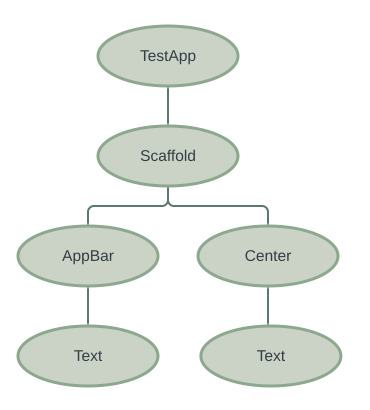
\includegraphics[scale=0.5]{stakeholder_matrix.png}
	\caption[Power/Interest Grid for Stakeholder-Analysis ]{Power/Interest Grid for Stakeholder-Analysis}
\end{figure}	

\section{System Context Diagram}
The greater environment in which a specific system or process functions is known as the system context. It covers all the outside variables and influences that affect the system's function, such as the stakeholders who are impacted by its operation, external systems, and processes with which it interacts and the policies and regulations that it must comply with. The system context can be determined using the previously performed stakeholder analysis. Determining the system context helps to get an understanding of which components interact with the system. This includes both the stakeholders and systems that influence the system.
The stakeholder groups of users and doctors can access the application via a smartphone. The developer and the database communicate with the system via direct code-based access.As already described in the APIs section, the database is filled with data from the ApiMedic API. The filling of the database will take place outside the system, in the form of a Python script (Jupyter Notebook). There surely are some aspects about privacy policy and the security of personal data of the users, especially during the verification process of the doctors. Since, in context of this bachelor thesis, the application will not be launched on the PlayStore these aspects are neglected in the system context.

\begin{figure}[h!]
	\centering
	\includegraphics[scale=0.65]{system_context.png}
	\caption[System Context Diagram ]{System Context Diagram}
\end{figure}

\section{User Requirements Specification}
The requirements for an application can be divided into three categories: functional requirements, non-functional requirements and optional requirements. In this section, the different types of requirements are considered and created project-specifically.

\subsection{Optional Requirements}
As the name suggests, optional requirements of an application consist of requirements that do not necessarily have to be implemented.
\begin{table}[H]
	\begin{center}
		\scriptsize
		\def\arraystretch{2}%
		\begin{tabular}{ c|l }
			\hline
			\textbf{ID} & \textbf{Description}  \\
			\hline
			OR1 & The application should make it possible to save and download a diagnosis in PDF format  \\
			\hline
			OR2 & The application should make it possible for a user to save tips on a favorites list  \\
			\hline	
		\end{tabular}
		\normalsize
	\end{center}
	\caption{Optional Requirements}
\end{table}
\subsection{Functional Requirements}
Functional requirements are the specific capabilities, behaviors, and features that a system must have. They describe what the system must do in order to be considered successful, and provide a basis for evaluating the system's performance and functionality.
\begin{table}[H]
	\begin{center}
		\scriptsize
		\def\arraystretch{2}%
		\begin{tabular}{ c|l}
			\hline
			\textbf{ID} & \textbf{Description}  \\
			\hline
			FR1 & The application must allow the user to switch between the diagnostics and the advices view  \\
			\hline
			FR2 & The application must offer the user the option of being able to verify themselves as a doctor  \\
			\hline
			FR3 & The application must offer a doctor the opportunity to log in  \\
			\hline
			FR4 & The application must offer a doctor the opportunity to add a new record in the database  \\
			\hline
			FR5 & The application must offer a doctor the possibility of editing data records in the database  \\
			\hline
			FR6 & The application must allow a user to start a new diagnosis  \\
			\hline
			FR7 & The application must enable a user to save a diagnosis  \\
			\hline	
			FR8 & The application must enable a user to view his saved diagnoses again  \\
			\hline
			FR9& The application must allow a user to abort his diagnostic procedure at any time \\
			\hline
			FR10 & The application must allow a user to delete saved diagnoses  \\
			\hline
			FR11 & The application must allow a doctor to abort adding or editing data at any time\\
			\hline
		\end{tabular}
		\normalsize
	\end{center}
	\caption{Functional Requirements}
\end{table}

\subsection{Non-functional Requirements}
After the functional requirements have been determined, the non-functional requirements are now considered. Non-functional requirements can be described by not dealing with the direct interaction of a user with the application, but with the system-specific properties. This includes, for example, the reliability of the application, but also safety aspects. [Buch google]
\begin{table}[H]
	\begin{center}
		\scriptsize
		\def\arraystretch{2}%
		\begin{tabular}{ c|l }
			\hline
			\textbf{ID} & \textbf{Description}  \\
			\hline
			NFR1 & The application must make correct diagnoses  \\
			\hline
			NFR2 & The application must be usable for patients without registration  \\
			\hline
			NFR3 & The application should have a graphical interface that can be used intuitively  \\
			\hline	
		\end{tabular}
		\normalsize
	\end{center}
	\caption{Non-Functional Requirements}
\end{table}


\section{Use Cases}
The architectural goal of the application is to be designed to provide an optimal user experience for both, patients and doctors. In order to ensure this, it is necessary to determine, before the actual development, which use cases the software has to cover, i.e. the externally visible interactions of the users with the system. This ensures that the application meets the wishes of the users and that they actually use the application. In addition, possible ambiguities are revealed and required data structures are determined. Possible problems that may arise during use of the application are most likely to be found during the process and technical solutions can then be worked out. Experience has shown that use cases also make it easier for a developer to create the objects that have to be created with an object-oriented programming language in the early development process more precisely and to recognize and implement inheritance options at an early stage. Some use cases can be identified from the functional and optional requirements set out above. Figure 3.3 shows the resulting use case diagram, which has been shortened to the most relevant use cases. 

\begin{figure}[h]
	\centering
	\includegraphics[scale=0.6]{use_case_diagram.png}
	\caption[Use Case Diagram]{Use Case Diagram}
\end{figure}
\noindent
The use cases are described in detail in the following sections. The resulting use case tables for each of them can be found in the appendix [].

\subsection{Get Diagnosis}
The first use case is described by the fact that a user would like to receive a diagnosis \textbf{[FR6]}. The actors who can carry out this use case are both patients, i.e. normal users, and doctors. In this application, doctors represent a subclass of users. In order to start the disease determination, the trigger, which will be implemented in the form of a button, must be pressed. The system then responds by displaying the view to enter and specify symptoms. As soon as the actor has finished specifying the symptoms, the system calculates the possible diseases and displays them to the actor in the form of a diagnosis. The actor now has the opportunity to decide whether he wants to end the use case by exiting the diagnostic view or saving the diagnosis \textbf{[FR7]}, which is indicated by pressing the save button. The system then saves the diagnosis. Optionally, the actor should also be able to save the diagnosis as a PDF on his device \textbf{[OR1]}. During the process, the user has the option to cancel the symptom statement at any time, which ends the use case by returning to the main page of the application \textbf{[FR10]}.

\subsection{Review Received Diagnoses}
After the user has received his diagnosis, he should be able to look at old diagnoses again \textbf{[FR8]}. The prerequisite for seeing such a diagnosis is that the actor has previously saved it, when the diagnosis was made. A view is provided in the application in which saved diagnoses are displayed in a list. Clicking on such a diagnosis starts the use case, whereupon the system opens the detailed view of the diagnosis. The use case is ended by clicking on the back button provided for this purpose. While the diagnosis is being viewed, the user has the option of deleting the selected diagnosis, which is triggered by clicking on the icon provided for this purpose and is answered by deleting the diagnosis from the system. In this use case, too, the user is given the opportunity to save his diagnosis as a PDF \textbf{[OR1]}, the procedure for this corresponds to that of the "Get Diagnosis" use case.

\subsection{Login}
As already mentioned in the project goal, doctors should be given the opportunity to log into the application \textbf{[FR3]}. The trigger for the use case is the click on the login button. Once the button is pressed, the application will display the login page. There, the actor has the opportunity to enter his credentials, whereupon the system checks whether these are stored in the database. Should the result be positiv, the doctor will be logged in and the system will display the doctor's dashboard. The prerequisite, for the use case to be carried out without errors, is that the doctor has been able to verify himself as such beforehand \textbf{[FR2]}. If this has not yet happened, the user has the opportunity to click on the verify button, where he will be prompted to carry out this process and will be logged in if it is successful. Should it be not successfull, because the user can not verify himself as a doctor, the system will continue showing error messages to the acteur.  If the doctor is verified, but the system cannot find the entered credentials, an error message is displayed by the application and the user, suspecting that the credentials have been entered incorrectly, is asked to check his user data and try again after making a correction.

\subsection{Add Data}
Provided that he is logged in, a doctor can now add data to the database \textbf{[FR4]}. In order to do this, he must press the button provided for this purpose. The system then displays the blank template for a data record, in which the doctor can enter the data he wants to add. As soon as he has done this and pressed the confirm button, the system adds the data record to the database and saves it in his data list as well. If the actor presses the confirm button without entering anything in each data field, the application will display an error notification on the screen, prompting the user to fill in all data fields. If the user wishes to cancel the process, he is free to press the button provided for this at any time, whereupon the system closes the view and the use case ends \textbf{[FR11]}. 

\subsection{Edit Data}
In addition to the functionality to create new datasets, the doctor should be able to expand and edit existing datasets \textbf{[FR5]}. The structure of this use case is similar to the previously described use case of adding new data. The doctor must first be in the view in which all existing data records are displayed in list format. There he has the opportunity to click on one of these data sets, which signals to the system that it must now display the editing screen for the selected data set. In this view, the doctor can now make the desired changes and press the confirm button. The application will then update the record in the database and the use case will be terminated. As before when adding new data records, the doctor has the option to end the process at any time \textbf{[FR11]}.

\subsection{Get Tips and Tricks for Symptoms and Diseases}
The final use case worth mentioning is viewing advice on illnesses \textbf{[FR1]}. A user has the option to go to the view for all advice that Doctors have uploaded. Once he's navigated there and the system shows the predicted view, he can click on one of the pieces of advice there and it will be shown to him in detail. Optionally, the user can save the advice as a favorite by clicking on the button provided for this purpose \textbf{[OR2]}. 

\section{Domain Model}
Domain modeling is a major modeling topic in Agile development at scale because there is frequently a gap between comprehending the issue domain and the interpretation of requirements. It depicts the solution as a collection of domain objects that collaborate to satisfy system-level scenarios. [internetseite SAFe] The quintessence of the object-oriented analysis step is the decomposition of a domain into problem-relevant concepts or objects. A domain model is a visual representation of the problem-relevant domain classes of a domain. With the help of UML notation, a domain model is represented by a set of class diagrams in which no operations are defined, it presents a conceptual perspective and can show domain objects or classes, as well as associations between domain classes and attributes of domain classes. [UML 2 Buch]  Domain modeling is a major modeling topic in Agile development at scale because there is frequently a gap between comprehending the issue domain and the interpretation of requirements. Identifying domain entities and their connections, derived from a grasp of system-level requirements, offers a good foundation for understanding and supports practitioners in designing systems for maintainability, testability, and incremental development. [internetseite SAFe] Finding conceptual classes by recognizing substantive phrases is an effective technique to domain modeling. [Buch UML2]

\begin{itemize}
	\item A person is a \textbf{user} of the application.
	\item A \textbf{user} chooses a \textbf{body part}.
	\begin{itemize}
		\item A \textbf{body part} can be associated with different \textbf{symptoms}.
		\item A \textbf{user} selects a \textbf{symptom} and specifies the selected symptom by narrowing down (selecting) \textbf{proposed symptoms}, the \textbf{time of occurrence} and the \textbf{symptom intensity}. The information obtained is summarized as a textbf{user-specified symptom}.
	\end{itemize}
	\item One or more \textbf{user-specified symptoms} lead to the calculation of one or more possible \textbf{diseases}.
	\begin{itemize}
		\item A \textbf{disease} has different \textbf{symptoms}.
	\end{itemize}
	\item A \textbf{diagnosis} consists of one or more \textbf{diseases}.
	\item \textbf{Doctors} are special \textbf{users} of the application.
	\item \textbf{Doctors} can add/edit \textbf{advices}, \textbf{symptoms}, \textbf{body parts} and \textbf{diseases}.
	\item \textbf{Users} can view \textbf{advices}.  
\end{itemize}
\noindent
The information just obtained makes it easier to create the domain model. The entities user, symptom, user-specified symptom, body part, diseases, doctor, advice and diagnosis can already be recognized. Based on that information a domain model can be created. 
\begin{figure}[H]
	\centering
	\includegraphics[scale=0.2]{domain_model.png}
	\caption[Domain Model]{Domain Model}
\end{figure}
\noindent
Based on the domain model and the previously obtained information, the database development can now be started. Later on, the chapter optimizations also addresses some aspects that have been neglected at the moment.

